\subsection{Problem definition}

\begin{figure}[h]
\centering
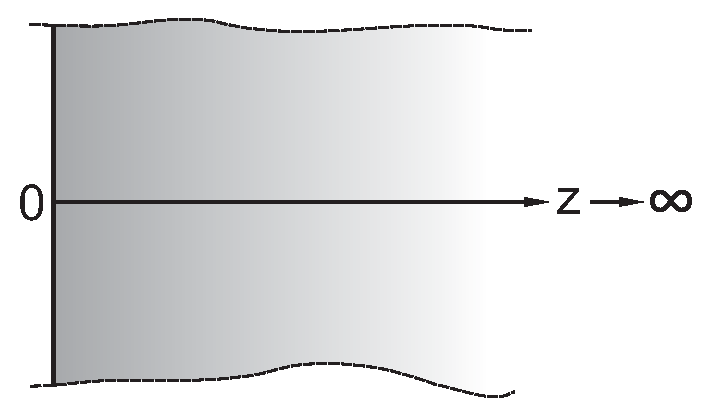
\includegraphics[width=0.5\textwidth]{T/figures/LHD.eps}
\caption{\label{figLHD}One side limited domain in cartesian coordinates.}
\end{figure}
%%%%%%%%%%%%%%%%%%%%%%%%%%%%%%%%%%%%%%%%%%%%%%%%%%%%%%%%%%%%%%%%%%%%%%%%%%%%%%%%%%%%%%%%
\subsection{Analytical solution}

The one dimensional heat transport in a domain limited just by one side can be derived by \eqref{eqn:lhd}
\begin{equation}
T(x,t) = T_0 \operatorname{erfc} \left(\frac{x}{\sqrt{4\alpha t}}\right),
\label{eqn:lhd}
\end{equation}
where $T_0$ is the initial temperature and $\alpha = \lambda/c\rho$ is the heat diffusivity coefficient of the used material.

%%%%%%%%%%%%%%%%%%%%%%%%%%%%%%%%%%%%%%%%%%%%%%%%%%%%%%%%%%%%%%%%%%%%%%%%%%%%%%%%%%%%%%%%
\subsection{Numerical solution}
\subsubsection{Model setup}

The numerical model consists of 60 line elements connected by 61 nodes along the z-axis (figure \ref{fig-ms-lhd}). The distances of the nodes $\Delta z$ is one meter. At $z=\unit[0]{m}$ there is a constant temperature boundary condition. 
\begin{figure}%[img-msldh]
%\label{img-msldh}
\centering
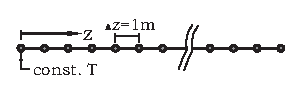
\includegraphics[width=0.5\textwidth]{T/figures/ms-lhd.eps}
\caption{\label{fig-ms-lhd}Spatial discretisation of the numerical model.}
\end{figure}
%%%%%%%%%%%%%%%%%%%%%%%%%%%%%%%%%%%%%%%%%%%%%%%%%%%%%%%%%%%%%%%%%%%%%%%%%%%%%%%%%%%%%%%%%%%%%%%%%%%%
\subsubsection{Parameters}

The material properties for this model setup are given in Tab.~\ref{tab-ldhp}.
%\begin{table}[tab-ldhp]
%\centering
%\label{tab-ldhp}
%\caption{Material properties}
%\begin{tabular}{|c|l|l|}
%\hline
%symbol & quantity & value \\
%\hline
%$\rho$   & density of the solid & 2500  kg$\cdot$m$^{-3}$ \\			
%\hline
%$c$	     & thermal capacity	    & 1000  J$\cdot$kg$^{-1}\cdot$K$^{-1}$ \\
%\hline
%$\lambda$ & thermal conductivity	& 3.2  W$\cdot$m$^{-1}\cdot$K$^{-1}$ \\
%\hline
%\end{tabular}
%\end{table}
\begin{table}[h]%[tab-ldhp]
\caption{\label{tab-ldhp}Material properties.}
\begin{center}
\begin{tabular}{ll}
\toprule
parameter & value \\
\midrule
density $\rho$ of the solid & 2500  kg$\cdot$m$^{-3}$ \\			
heat capacity	$c$	    & 1000  J$\cdot$kg$^{-1}\cdot$K$^{-1}$ \\
thermal conductivity $\lambda$	& 3.2  W$\cdot$m$^{-1}\cdot$K$^{-1}$ \\
\bottomrule
\end{tabular}
\end{center}
\end{table}
Using these values, the outcome for the heat diffusivity constant $\alpha = \lambda/c\rho$ in \eqref{EqHT} is $\alpha=1.28\cdot$10$^{-6}m^2/s$.
%%%%%%%%%%%%%%%%%%%%%%%%%%%%%%%%%%%%%%%%%%%%%%%%%%%%%%%%%%%%%%%%%%%%%%%%%%%%%%%%%%%%%%%%%%%%%%%%%%%%%%%%
\subsubsection{Temporal discretisation}

The \textit{Neumann} stability criteria has to be restrained so that the temperature gradient can't be inverted by diffusive fluxes. Using \eqref{eqn:ne-ldh} the best time step can be estimated by
\begin{equation}
\operatorname{Ne} = \frac{\alpha\Delta t}{(\Delta z)^2}\leq\frac{1}{2}.
\label{eqn:ne-ldh}
\end{equation}
With $\Delta z=\unit[1]{m}$ and $\alpha=\unit[1.28 \cdot 10^{-6}]{m^2/s}$ the outcome for the timestep is $\Delta t\leq \unit[390.625]{s}$ or 4.5 days respectively.
%%%%%%%%%%%%%%%%%%%%%%%%%%%%%%%%%%%%%%%%%%%%%%%%%%%%%%%%%%%%%%%%%%%%%%%%%%%%%%%%%%%%%%%%
\subsection{Results}

%The following figure show the comparison of the solution of \eqref{eqn:lhd} and the numerical simulation results. Fig.~\ref{fig-lhd-all} shows the temperature distribution along the model domain after 2 months, 1 year, 2 years and 4 years.
The following figure (Fig.~\ref{fig-lhd-all}) show the comparison of the solution of \eqref{eqn:lhd} and the numerical simulation results. It is demontrated the temperature distribution along the model domain after 2 months, 1 year, 2 years and 4 years.
\begin{table}%[]
\caption{Benchmark deposit.}
\begin{center}
\begin{tabular}{lll}
\toprule
Deposit & Version & Date \\
\midrule
T$\backslash$TDiff$\backslash$TDiff & 4.7.03 & Jun.~2008 \\
\bottomrule
\end{tabular}
\end{center}
\end{table}
\begin{figure}%[img-lhd-all]
\centering
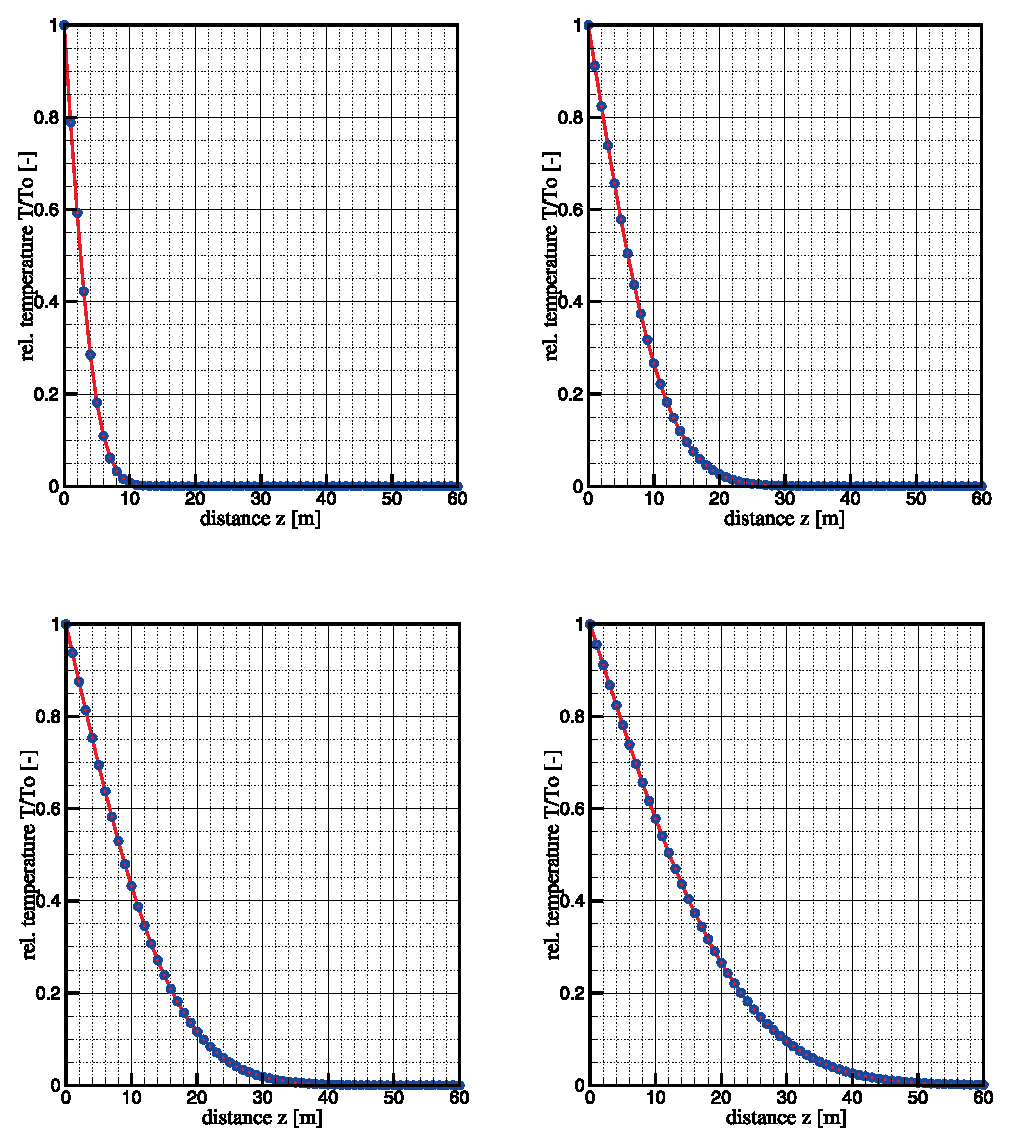
\includegraphics[width=0.9\textwidth]{T/figures/lhd-all.eps}
\caption{\label{fig-lhd-all}Temperature distribution along the z-axis after 2 months, 1 year, 2 years and 4 years (from top left to down right).}
\end{figure}
%\clearpage